\section{Gap Algorithm Additional Graphs}
\label{sec:extra_graphs}

In this appendix the run-time performance of the DFA-Gap algorithm and the regular expression variant will be explored further. The values for Perl and Python are omitted from these graphs due to their out-sized values.

\subsection{DFA-Gap Run-time Progression}
\label{subsec:dfa-gap-runtimes}

Figure~\ref{fig:graph:dfa-runtimes} showed the run-times for the DFA version, with each language ``stacking'' their times for side-by-side comparison. Here, the increase in run-time as $k$ increases is plotted as a different view of that data.

\begin{figure}[h]
	\centering
	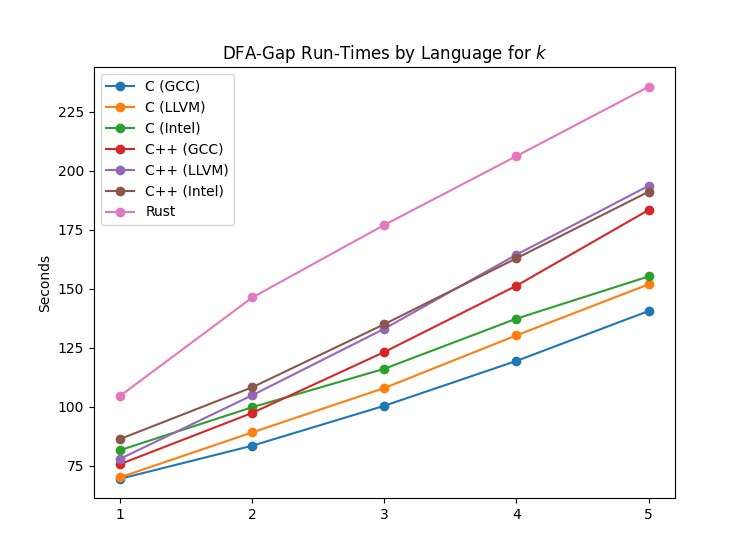
\includegraphics[width=0.85\textwidth]{figures/k_runtimes-dfa_gap.png}
	\caption{Plots of run-times for DFA-Gap by values of $k$}
	\label{fig:graph:k_runtimes-dfa_gap}
\end{figure}

The seven plots are all distinguishable from each other, with the GCC C line (blue) being the lowest and the Rust (pink) line the highest. Between these two, the remaining C varieties and all three C++ varieties have very similar slopes (except for Intel C, green, which is increasing more slowly than the others, and might potentially cross the GCC C line around $k=7$ were the experiments taken that far).

What is most interesting in this set of plots is that each plot itself is functionally linear. The initial impression of this algorithm was that it would most likely show a time-complexity close to O($(m+k)n$), and indeed in section~\ref{subsec:regexp_variant} a stated goal of the regular expression variant was to keep within that range. Given that the experiment data was very uniform in both the sequence lengths (``$n$'') and the pattern lengths (``$m$''), it is hard to extrapolate from this data whether this complexity estimate is accurate.

Further study of this algorithm that includes greater variety in pattern-length and sequence-length would be of great benefit to determining whether the complexity is truly O($(m+k)n$), closer to the basic O($mn$), or something closer to O($kmn$).

\subsection{Regexp-Gap Run-time Progression}
\label{subsec:regexp-gap-runtimes}

For the regular expression version, figure~\ref{fig:graph:regexp-runtimes} originally showed the stacked impression of the run-times by language. The following graph shows the same data as above, with each line representing a language and the values growing to the right with increasing $k$.

\begin{figure}[h]
	\centering
	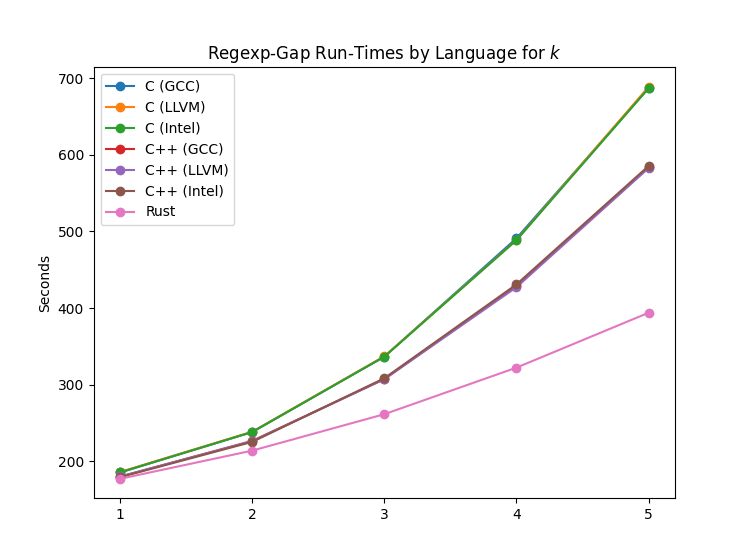
\includegraphics[width=0.85\textwidth]{figures/k_runtimes-regexp.png}
	\caption{Plots of run-times for Regexp-Gap by values of $k$}
	\label{fig:graph:k_runtimes-regexp}
\end{figure}

In this set of plots the performance of Rust is clear as the bottom-most (pink) line. What appears to be two additional lines, however, is actually two groups of nearly-identical times. The top-most plot is actually the lines for LLVM C and Intel C almost completely overlapping. And the middle line is the overlapping of GCC C and all three C++ varieties.

This is actually rather expected in terms of results, as all of these experiments were just basic wrappers around the PCRE2 engine. It is the performance of Rust that is the most noteworthy, as it appears at first glance to be almost linear while the C and C++ plots are clearly parabolic. However, the Rust curve does follow a very shallow quadratic polynomial path.

Further study here could also focus on varying lengths of sequences and patterns, but also look into how the value of $k$ influences the curve itself.
